\def\mytitle{OPTIMIZATION USING PYTHON}
\def\myauthor{V.GOKULKUMAR}
\def\contact{velicharlagokulkumar@gmail.com}
\def\mymodule{Future Wireless Communication (FWC)}
\documentclass[10pt, a4paper]{article}
\usepackage[a4paper,outer=1.5cm,inner=1.5cm,top=1.75cm,bottom=1.5cm]{geometry}
\twocolumn
\usepackage{graphicx}
\graphicspath{{./images/}}
\usepackage[colorlinks,linkcolor={black},citecolor={blue!80!black},urlcolor={blue!80!black}]{hyperref}
\usepackage[parfill]{parskip}
\usepackage{lmodern}
\usepackage{tikz}
	\usepackage{physics}
%\documentclass[tikz, border=2mm]{standalone}
%\usepackage{karnaugh-map}
%\documentclass{article}
\usepackage{tabularx}
\providecommand{\sbrak}[1]{\ensuremath{{}\left[#1\right]}}
\providecommand{\brak}[1]{\ensuremath{\left(#1\right)}}
\usepackage{enumitem}
\usetikzlibrary{calc}
\usepackage{amsmath}
\usepackage{amssymb}
\renewcommand*\familydefault{\sfdefault}
\usepackage{watermark}
\usepackage{lipsum}
\usepackage{xcolor}
\usepackage{listings}
\usepackage{float}
\usepackage{titlesec}
\providecommand{\mtx}[1]{\mathbf{#1}}
\titlespacing{\subsection}{1pt}{\parskip}{3pt}
\titlespacing{\subsubsection}{0pt}{\parskip}{-\parskip}
\titlespacing{\paragraph}{0pt}{\parskip}{\parskip}
\newcommand{\figuremacro}[5]{
    \begin{figure}[#1]
        \centering
        \includegraphics[width=#5\columnwidth]{#2}
        \caption[#3]{\textbf{#3}#4}
        \label{fig:#2}
    \end{figure}
}
\usepackage{caption}
\newcommand{\myvec}[1]{\ensuremath{\begin{pmatrix}#1\end{pmatrix}}}
\let\vec\mathbf
\lstset{
frame=single, 
breaklines=true,
columns=fullflexible
}
\thiswatermark{\centering \put(181,-119.0){
\includegraphics[scale=0.13]{iith_logo3}} }
\title{\mytitle}
\author{\myauthor\hspace{1em}\\\contact\\FWC22034\hspace{6.5em}IITH\hspace{0.5em}\mymodule\hspace{6em}Assignment}
\begin{document}
	\maketitle
	\tableofcontents
   \section{Problem}
Find the absolute maximum value and the absolute minimum value of the following
functions in the given intervals:
\begin{align}
    f(x) &= 4x-\frac{1}{2}x^2 , x \in \sbrak{-2,\frac{9}{2}}
\end{align}
\section{Solution}
A function f(x) is said to be convex if following inequality is true for $\lambda \in [0,1] :$  \label{opt/2/1/a/lemma1}
\begin{align}
    \lambda f(x_1) + (1-\lambda)f(x_2) \geq f(\lambda x_1 + (1-\lambda)x_2)
    \label{eq:2}
\end{align}

Checking convexity of $f(x)$ :
\begin{equation}
\begin{aligned}
    &\lambda\brak{4x_1-\frac{1}{2}x_1^2} + (1-\lambda)\brak{4x_2-\frac{1}{2}x_2^2} \geq \\
    &4\brak{\lambda x_1 + (1-\lambda)x_2} - \frac{1}{2}\brak{\lambda x_1 + (1-\lambda)x_2}^2
\end{aligned}
\end{equation}
\begin{align}
        x_1^2\brak{\frac{\lambda^2-\lambda}{2}}+x_2^2\brak{\frac{\lambda^2-\lambda}{2}}+2x_1x_2\brak{\frac{\lambda-\lambda^2}{2}} &\geq 0 \\
        \brak{\frac{\lambda^2-\lambda}{2}}\brak{x_1^2+x_2^2-2x_1x_2} &\geq 0 \\
        -\frac{1}{2}\lambda\brak{1-\lambda}\brak{x_1-x_2}^2 &\geq 0 \\
        \implies \frac{1}{2}\lambda\brak{1-\lambda}\brak{x_1-x_2}^2 &\leq 0 \label{eq:7}
\end{align}
Equation \eqref{eq:7} holds true for all $\lambda\in(0,1)$. Hence the given function f(x) is concave
 For a general quadratic equation
\begin{align}
    f(x)=ax^2+bx+c
\end{align}

\begin{enumerate}
\item For Maxima : \\
    Using gradient ascent method,
\begin{align}
    x_n=x_{n-1}+\mu\frac{df(x)}{dx} \label{eq:9}
    \end{align}
    \begin{align}
    \frac{df(x)}{dx}=4-x \label{eq:10}
\end{align}
After substituting \ref{eq:10} in \ref{eq:9} we get:
\begin{align}
    x_n=x_{n-1}+\mu(4-x_{n-1})\label{eq:11}
\end{align}
In equation \eqref{eq:9}, $\mu$ is a variable parameter known as step size. $x_{n+1}$ is the next position. The plus sign refers to the maximization part of gradient ascent. Assume, $\mu=0.001$, Taking $x_0=-2$,precision= 0.00000001 and following the above method, we keep doing iterations until $x_{n+1}-x_{n}$ becomes less than the value of precision we have chosen.
\begin{enumerate}
	\item The absolute maxima occurs at
	3.9999900196756437
	\begin{align}
    x_n=4
\end{align}
	\item The value of f(x) at maxima is 
	7.999999999950196
\end{enumerate}
    \begin{align}
        \boxed{\text{Maxima} = 7.999999999950196 \approx 8 }\\
        \boxed{\text{Maxima Point} = 3.9999900196756437 \approx 4}
    \end{align}
    Hence, The maxima value of $f(x)$ at $x=4$ is 8.
    
   \begin{figure}[!ht]
    \centering
    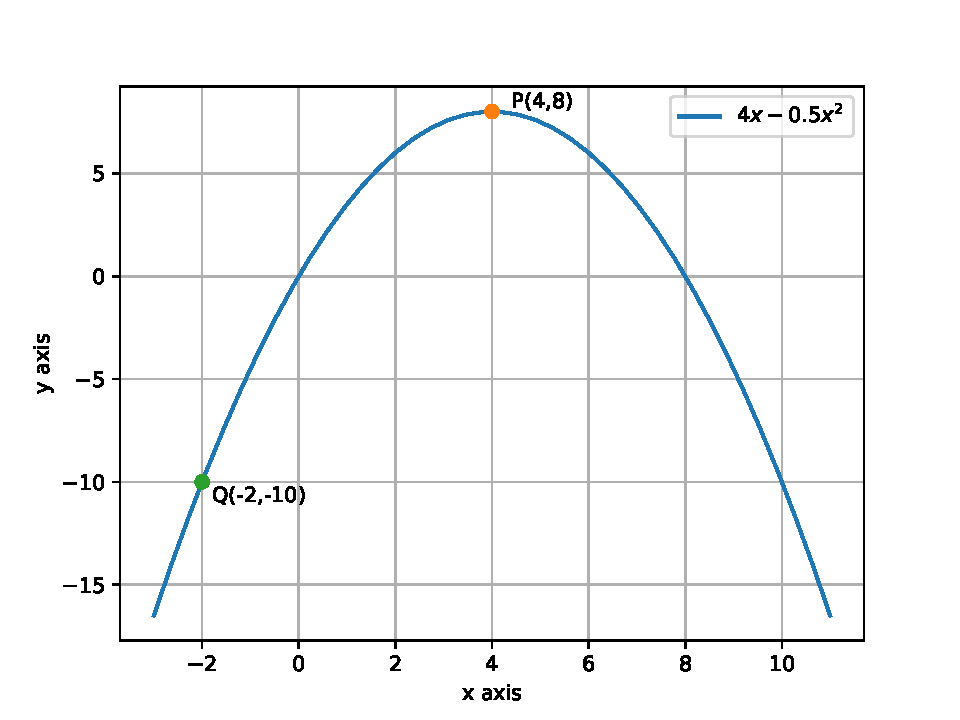
\includegraphics[width=\columnwidth]{optimize2.pdf}
    \caption{$f(x)=4x-0.5x^2$}
    \label{fig:1}
\end{figure}
\item  For Minima : 
    Critical point is given by
    \begin{align}
       \frac{df(x)}{dx} &= 0 \\
        \implies x &= 4
    \end{align}
    
    and,end points are $x=-2$ and $x=4.5$ .
    \begin{table}[!ht]
    \centering
    \begin{tabular}{|c|c|}
       	\hline
	$x$&$f(x)$\\
	\hline
	-2 & -10 \\
	\hline
	4&8\\
	\hline
	4.5&7.875\\
	\hline
    \end{tabular}
 \caption{Value of $f(x)$}
    \label{tab:table1}
\end{table}
Using table\ref{tab:table1},
    \begin{align}
        \boxed{\text{Minima} = -10}\\
        \boxed{\text{Minima Point} = -2}
    \end{align}
    Hence, The minima value of $f(x)$ at $x=-2$ is -10.
\end{enumerate}

The following python code computes the maxima,minima value as plotted in Fig. \ref{fig:1}. 
\begin{center}
\fbox{\parbox{8.5cm}{\url{https://github.com/velicharlagokulkumar/FWC_module1/blob/main/optimization/other/codes/optimize2.py}}}
\end{center}


\end{document}
